\documentclass{article}
\usepackage[utf8]{inputenc}
\usepackage{graphicx}
\usepackage{geometry}
\usepackage{amsmath}
\usepackage{amsfonts}
\usepackage{float}
\usepackage{caption}
\usepackage{subcaption}
\usepackage{enumitem}

\geometry{left=25mm, top=25mm, right=25mm, bottom=25mm}

\title{PHY407 Lab 10}
\author{Pierino Zindel (1002429703) and Hayden Johnson (1002103537)}
\date{November 23, 2018}

\begin{document}

\maketitle

\noindent \textbf{Distribution of work:} Question 1 was completed by Pierino. Questions 2 and 3 were completed by Hayden.

\section{Brownian Motion and Diffusion Limited Aggregation}

\section{Volume of a 10-dimensional Hypersphere}

We seek to compute the volume of a 10-dimensional hypersphere, using the Monte Carlo mean value integration method, and also to estimate the error of our calculated value relative to the true value.

We define an indicator function $f(x)$ which takes a value of one inside the sphere and value of zero outside of it. Then the volume of the sphere is given by:
\begin{equation}
	V = \int_{|x|\leq 1}f(x) dx
\end{equation}
Where $x \in \mathbb{R}^{10}$ and the integral is over all dimensions. Using the Monte Carlo mean value method, we consider a cubic integration region $[-1,1]^{10}$, which has a volume of $2^{10}$, and use a collection of $N$ randomly-generated points $x_i$ contained in the volume at which to evaluate $f$. The value of our integral (and thus the volume of the hypersphere) is then approximated by:
\begin{equation}
	I = \frac{2^{10}}{N}\sum_{i=1}^N f(x_i)
\end{equation}

The variance of the value of the function $f(x)$ is given by:
\begin{equation}
	\text{var}f = \langle f^2 \rangle - \langle f \rangle^2
\end{equation}
Where $\langle a \rangle$ represents the average value of the variable $a$. The variance of the sum of $f(x)$ over $N$ points is then $N\cdot\text{var}f$, and the standard deviation of the sum is $\sqrt{N\cdot\text{var}f}$. Hence the standard deviation of the volume is:
\begin{equation}
	\sigma = \frac{2^{10}}{N}\sqrt{N\cdot\text{var}f} = \frac{2^{10}\sqrt{\text{var}f}}{\sqrt{N}}
\end{equation}
And we take this standard deviation to be our estimate of the error in the calculated value of the volume.

The values of the volume and associated error output by the program are presented in table \ref{tab:q2}. The analytic value of the volume of a unit sphere in 10 dimensions is, according to Wikipedia, 2.550, and our calculated value is within our calculated error of this, suggesting that we have done the computation correctly.

\begin{table}[H]
	\centering
	\caption{Values of the volume of the hypersphere and error associated with the calculation as output by the program.}
	\label{tab:q2}
	\begin{tabular}{c|c}
		Quantity & Value \\
		\hline
		Volume & 2.567 \\
		Error & 0.051
	\end{tabular}
\end{table}

\section{Importance Sampling}

\subsection{Part a)}

We seek to evaluate the integral (\ref{eq:q3_a_integral}) a total of 100 times each using both the mean value and importance sampling Monte Carlo integration methods, and then plot the results in a histogram to characterize the behaviour of the methods.
\begin{equation}
	\label{eq:q3_a_integral}
	I = \int_0^1 \frac{x^{-1/2}}{1+e^x}dx
\end{equation}
We call the integrand function $f(x)$ where:
\begin{equation}
	f(x) = \frac{x^{-1/2}}{1+e^x}
\end{equation}

The computation of the integral using the regular mean value method is done using:
\begin{equation}
	\label{eq:q3_mv}
	I \approx \frac{b-a}{N}\sum_{i=1}^N f(x_i)
\end{equation}
Where the $x_i$ are drawn randomly from a uniform distribution.

For the importance sampling, we use a weighting function of $w(x) = x^{-1/2}$. The corresponding normalized probability density is:
\begin{equation}
	p(x) = \frac{w(x)}{\int_a^b w(x)dx} = \frac{x^{-1/2}}{\int_0^2 x^{-1/2}dx} = \frac{1}{2\sqrt{x}}
\end{equation}
To draw samples from the interval $[0,2]$ according to this distribution, we appeal to equation 10.7 from Newman, to see that:
\begin{equation}
	z = \int_a^x p(x)dx = \int_0^x \frac{dx}{2\sqrt{x}} = \sqrt{x} 
\end{equation}
Where $z$ are variables drawn from a uniform distribution. Hence the map from the uniform distribution to our required distribution is given by $x = z^2$.

We can now compute the value of the integral using importance sampling as:
\begin{equation}
	\label{eq:q3_is}
	I \approx \frac{1}{N}\sum_{i=1}^N \frac{f(x_i)}{w(x_i)} \int_a^b w(x)dx
\end{equation}
Where the $x_i$ are drawn from our non-uniform distribution described above.

Histograms of the values computed for the integral (\ref{eq:q3_a_integral}) using both methods are displayed in figure \ref{fig:q3_a}. It is quite clear from inspection that there is a larger spread in the calculated values using the mean value method than there is from the importance method; this is what we expect to see, since both methods were evaluated using the same number of points and the importance method is designed to produce a more accurate result by taking points preferentially from areas that are more important for capturing the behaviour of the integrand.

\begin{figure}[H]
	\centering
	\begin{minipage}{0.49\linewidth}
		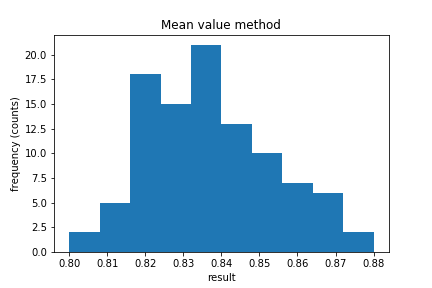
\includegraphics[width=\linewidth]{../images/q3_a_mv.png}
	\end{minipage}
	\begin{minipage}{0.49\linewidth}
		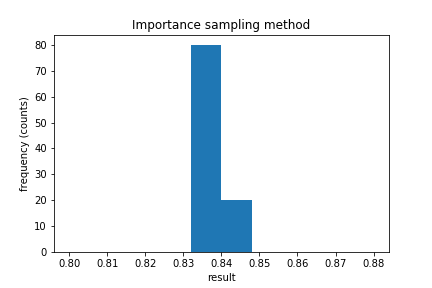
\includegraphics[width=\linewidth]{../images/q3_a_is.png}
	\end{minipage}
	\caption{Histogram of results for computation of the integral (\ref{eq:q3_a_integral}) using the mean value (left) and importance sampling (right) Monte Carlo methods 100 times.}
	\label{fig:q3_a}
\end{figure}

\subsection{Part b)}

We seek to evaluate the integral (\ref{eq:q3_b_integral}) a total of 100 times each using both the mean value and importance sampling Monte Carlo integration methods, and then plot the results in a histogram to characterize the behaviour of the methods.
\begin{equation}
	\label{eq:q3_b_integral}
	I = \int_0^{10} e^{-2|x-5|}dx
\end{equation}
Our integrand function $f(x)$ is given by:
\begin{equation}
	\label{eq:q3_b_f}
	f(x) = e^{-2|x-5|}
\end{equation}

The mean value method can be evaluated again using equation \ref{eq:q3_mv}, replacing the definition of $f(x)$ with equation \ref{eq:q3_b_f}.

For the importance sampling method, we use a Gaussian weighting function, which corresponds to an identical probability distribution, which are given by:
\begin{equation}
	\label{eq:q3_b_w}
	p(x) = w(x) = \frac{1}{\sqrt{2\pi}}e^{-(x-5)^2/2}
\end{equation}
We can then compute the integral using the importance sampling method by means of equation \ref{eq:q3_is}, replacing the pertinent definitions with those in equation \ref{eq:q3_b_w}, and noting that:
\begin{equation}
	\int_0^{10} w(x)dx = \int_0^{10} \frac{1}{\sqrt{2\pi}}e^{-(x-5)^2/2}dx \cong 1
\end{equation}

Histograms of the values computed for the integral (\ref{eq:q3_b_integral}) using both methods are displayed in figure \ref{fig:q3_b}. It is quite clear from inspection that, as in part a), there is again a larger spread in the calculated values using the mean value method than there is from the importance method; this is what we expect to see, since both methods were evaluated using the same number of points and the importance method is designed to produce a more accurate result by taking points preferentially from areas that are more important for capturing the behaviour of the integrand.

\begin{figure}[H]
	\centering
	\begin{minipage}{0.49\linewidth}
		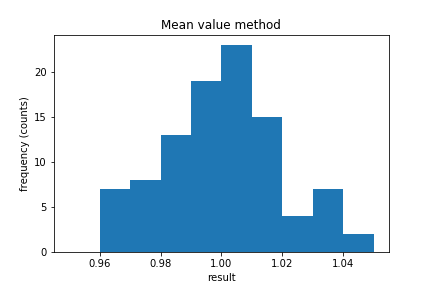
\includegraphics[width=\linewidth]{../images/q3_b_mv.png}
	\end{minipage}
	\begin{minipage}{0.49\linewidth}
		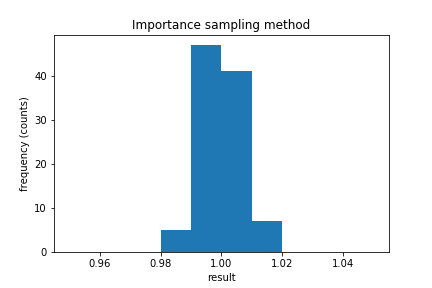
\includegraphics[width=\linewidth]{../images/q3_b_is.png}
	\end{minipage}
	\caption{Histogram of results for computation of the integral (\ref{eq:q3_b_integral}) using the mean value (left) and importance sampling (right) Monte Carlo methods 100 times.}
	\label{fig:q3_b}
\end{figure}


\end{document}